\chapter{Results}
\label{chapter:results}

In this chapter we present how the front-end application works from the user's standpoint and how the React components mutate upon browser events. In section \labelindexref{UI overview}{sec:ui-overview} we present how the UI looks and how its structured with the rendered components.

Next, in section \labelindexref{Edit Panel}{sec:edit-panel} we describe how the \texttt{GenericForm} components generate edit panels and how they are displayed.

Finally in the \labelindexref{Panel Nesting}{sec:panel-nesting} section we describe how the application renders the explored content trough the API.

\section{UI overview}
\label{sec:ui-overview}

In \labelindexref{Figure}{img:main-view} we present the rendered user interface and how the React components are structured after they are rendered using the Bootstrap framework and Flex CSS. It can also be seen that the parent component is the \texttt{FormBox} that encapsulates the other UI elements.

In the \texttt{Navbar} component the user uses a text input to pick or insert any API endpoint URI and then he can press the render button to trigger the initial AJAX GET call. 

On the server response the \texttt{FormList} is initialized with \texttt{GenericForm} components. In the example presented below we can see a list of six \texttt{GenericForm} components. Even if the first component looks different from the other five, the \texttt{AddForm} panel is in fact a \texttt{GenericForm}, which we will present in more detail in subsection \labelindexref{Add Panel}{sec:add-panel}.

The other \texttt{GenericForm} components describe a simple usage of an admin panel for a list of \texttt{Posts}. We can see that the \texttt{post} components feature info about the \texttt{title, content, author, id} and \texttt{creation\_date}. The panels also feature buttons for user interaction like editing or deleting. Next we will present the behavior of the post panels on user interaction and we will describe how the data inside is structured.

\begin{figure}[H]
	\centering
		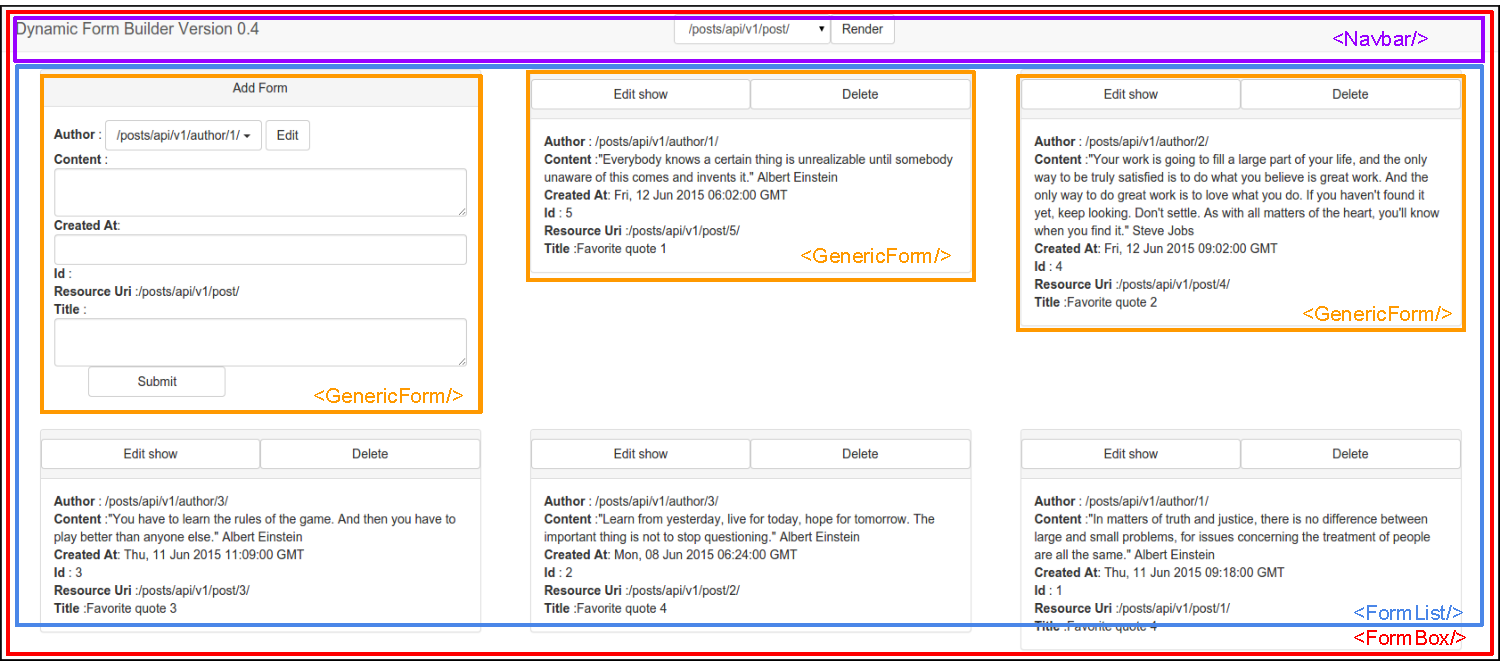
\includegraphics[scale=0.9, angle=90]{src/img/screenshot-app-0.pdf}
	\caption{User interface structure\label{img:main-view}}
\end{figure}

\section{Edit Panel}
\label{sec:edit-panel}

The \texttt{EditPanel} is the main component of the UI. It renders the data that is retrieved from the API regardless of its type. As described in the \labelindexref{GenericForm}{sub-sec:generic-form} section, the panel will have two states: \texttt{show} and \texttt{edit}. In \labelindexref{Figure}{img:panels} we present how does the \texttt{EditPanel} mutate when the user triggers a state change from \texttt{show} (default) to \texttt{edit} by pressing the \texttt{Edit show} button.

\begin{figure}[H]
	\centering
	\frame{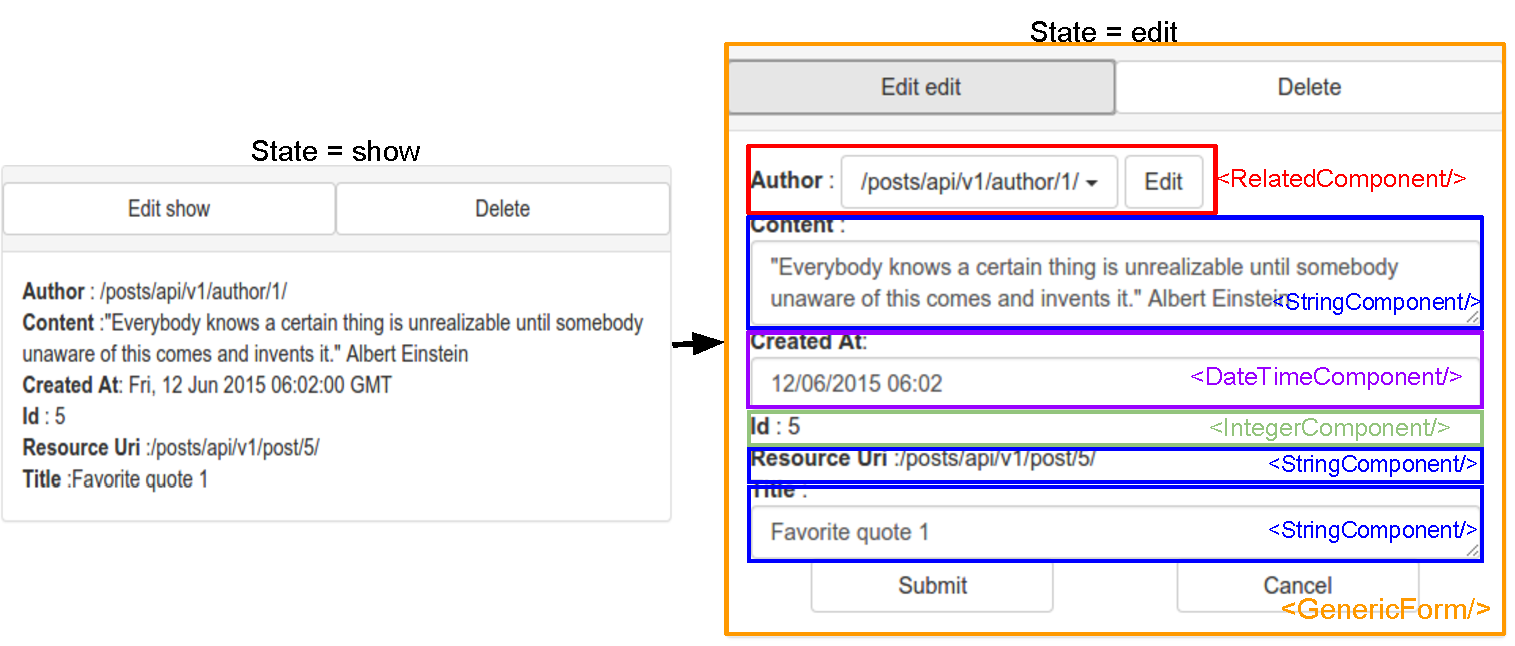
\includegraphics[scale=0.55]{src/img/panels2.pdf}}
	\caption{Edit panel states\label{img:panels}}
\end{figure}


In the right section of the figure above we describe the structure of the \texttt{GenericForm} component. In the \texttt{edit} state all components have a specific behavior described by the auto-generated html elements based on the \texttt{key:value} structured object properties as follows:

\begin{itemize}
	\item The \textbf{RelatedComponent} (in red) is structured as a string \texttt{key} (\texttt{Author}) followed by a \texttt{dropdown} component and an \texttt{Edit} button. When the \texttt{GenericForm} component changes state from \texttt{show} to \texttt{edit} the \texttt{dropdown} component is populated with data that describes the \texttt{key} object (in our case the Author). Finally, the \texttt{Edit} button triggers the exploration method in the \texttt{RelatedComponent} which we will present in more detail in the \labelindexref{Panel Nesting}{sec:panel-nesting} section.
	\item The \textbf{StringComponent} (in blue) appears multiple times and is represented by a string \texttt{key} (eg. \texttt{Content}) and a \texttt{textarea} HTML component. Also it can be seen that there are cases when the component will be \texttt{readonly} (in our case \texttt{Resource URI}) therefore the value will only be displayed as a \texttt{string}.
	\item The \textbf{IntegerComponent} (in green) has a similar structure with the \texttt{StringComponent} and in our case it also features a \texttt{readonly} mode.
	\item Finally the \textbf{DateTimeComponent} is composed of a string \texttt{key} (\texttt{Created At}) and a field that displays the date and time and on a \texttt{onClick} event initializes the Bootstrap Datepicker\footnote{\url{http://eonasdan.github.io/bootstrap-datetimepicker/}} component which is shown in \labelindexref{Figure}{img:date-time-panel}. The component adds a consistent look and experience to the application which is one of the main objectives of this project.
\end{itemize}
%\fig[scale=0.5]{src/img/date-time-panel.png}{img:date-time-panel}{DateTimeComponent in use}
\begin{figure}[H]
	\centering
	\frame{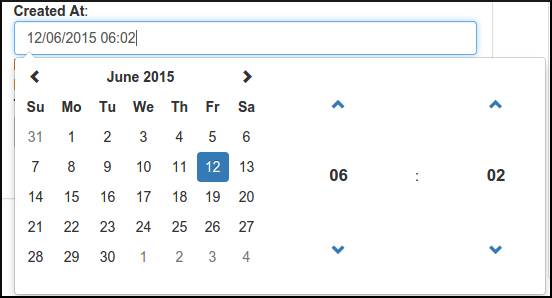
\includegraphics[scale=0.5]{src/img/date-time-panel.png}}
	\caption{DateTimeComponent in use\label{img:date-time-panel}}
\end{figure}


%consitent look and experience
\subsubsection{Add Panel}
\label{sec:add-panel}

The \texttt{AddPanel} component (also shown in \labelindexref{Figure}{img:main-view}) can be used by the user to submit a new \texttt{Post} entity to the database trough the REST API. This component is actually a \texttt{GenericForm} that receives an \texttt{optional} property from the \texttt{FormList} parent. On initialization with the optional property the component will not render the \texttt{Edit, Delete} and \texttt{Cancel} buttons. Also the \texttt{Add} component must receive an empty object from its parent to be able to render empty input components.

%\fig[scale=0.5]{src/img/add-panel.png}{img:add-panel}{Add panel component}

\section{Resource exploration}
\label{sec:panel-nesting}

\texttt{RelatedComponents} have the ability to explore the given URI path and auto-generate more UI components based on this action. As presented in the \labelindexref{Generic Form}{sub-sec:generic-form} section, when a user presses the \texttt{Edit} button it triggers an AJAX GET call on that specific resource. Once the data is retrieved it will generate another \texttt{GenericForm} component that has all the proprieties of a normal one. This specific behavior is presented in \labelindexref{Figure}{img:nesting}.


\begin{figure}[H]
	\centering
	\frame{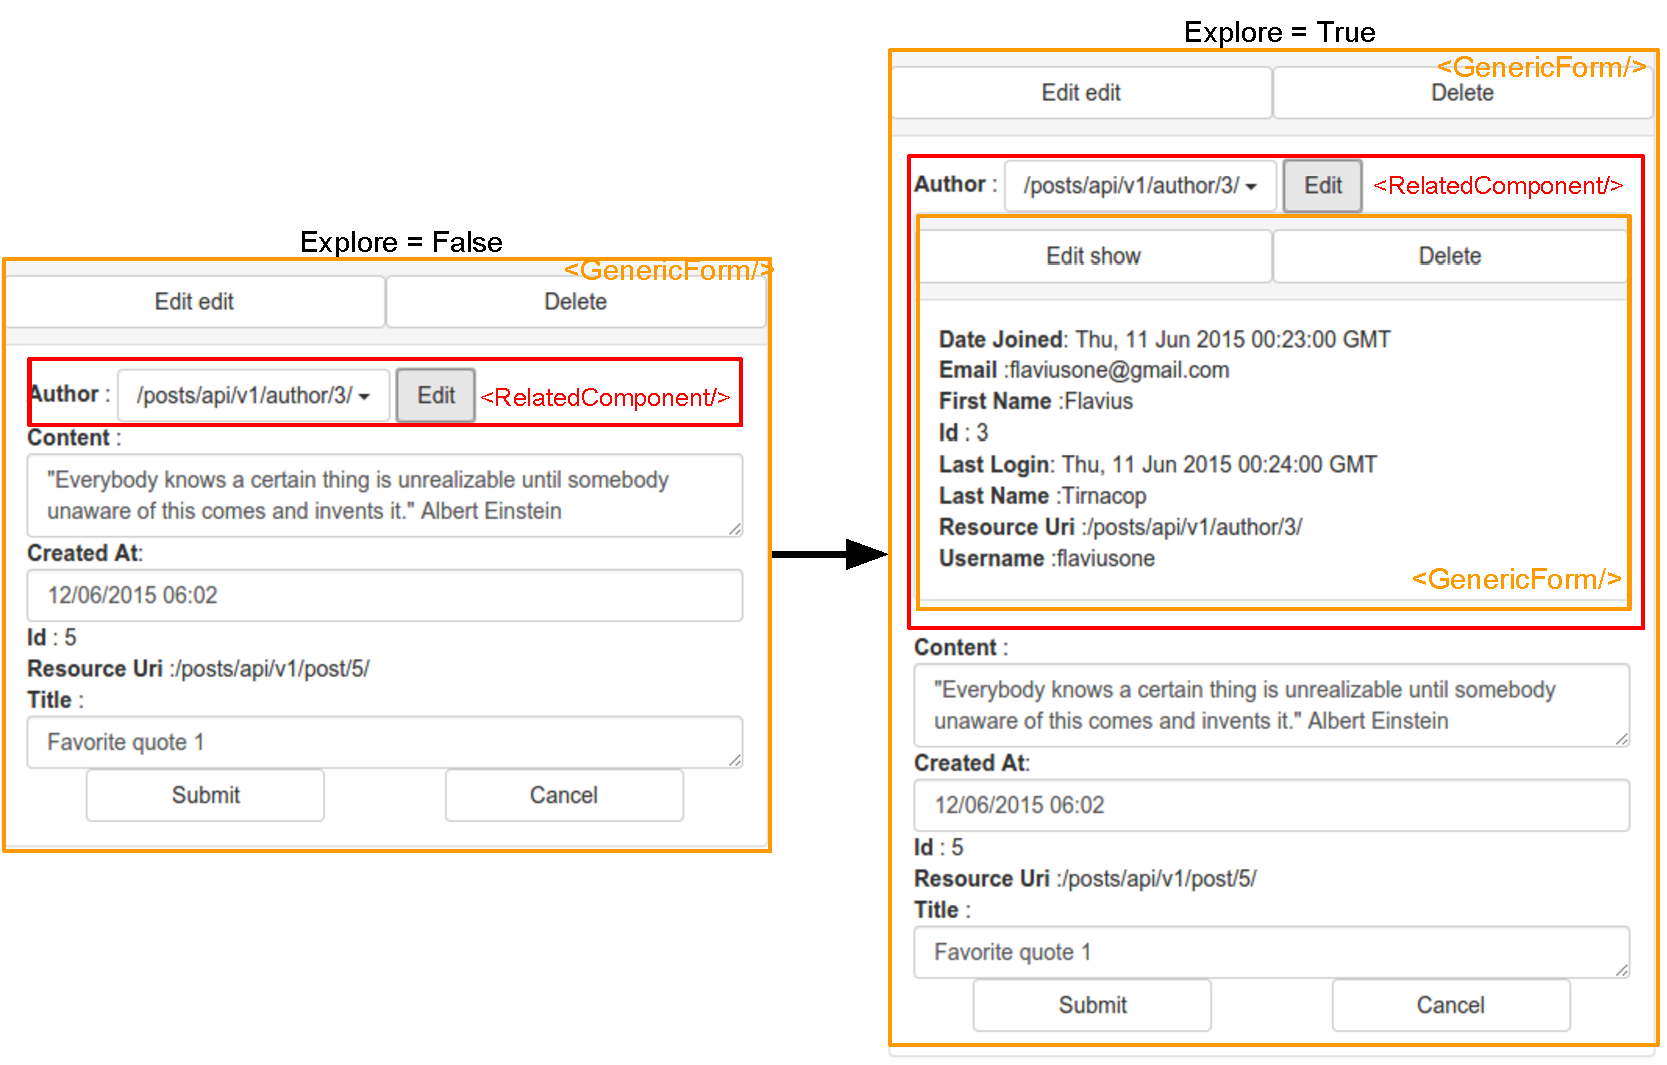
\includegraphics[scale=0.5]{src/img/nesting2.pdf}}
	\caption{Resource exploration\label{img:nesting}}
\end{figure}

%\fig[scale=0.50]{src/img/nesting2.pdf}{img:nesting}{PANELS}